%\begin{frame}
%	\vspace{-3em}
%	\begin{center}
%		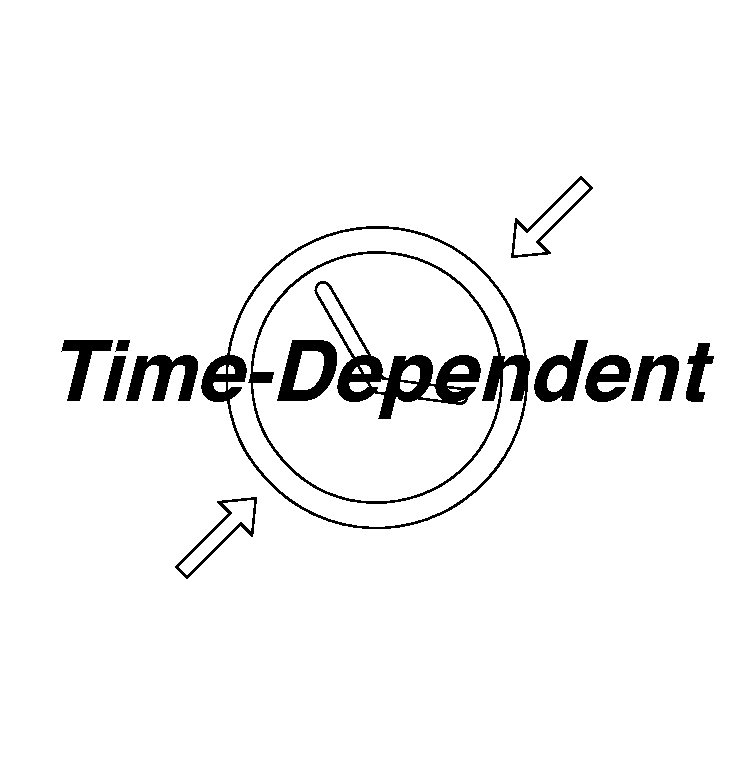
\includegraphics[width=.78\linewidth]{images/time-dependent/title.pdf} 
%	\end{center}
%\end{frame}


%\begin{frame}{Das Time-Dependent Modell}
%	\begin{itemize}
%		\item Denken wir zurück an das erste Beispiel...
%	\end{itemize}
%
%	\begin{center}
%		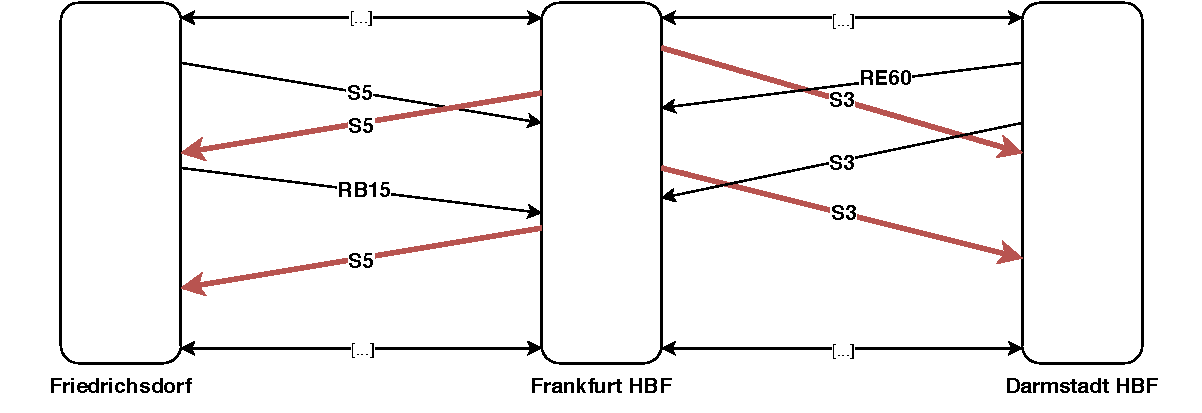
\includegraphics[width=\linewidth]{images/simple-approach-timed-3.pdf}
%	\end{center}
%\end{frame}


\begin{frame}{Das Time-Dependent Modell}
	\begin{itemize}
		\item Bauen wir das Beispiel vom Anfang etwas um...
	\end{itemize}

	\begin{center}
		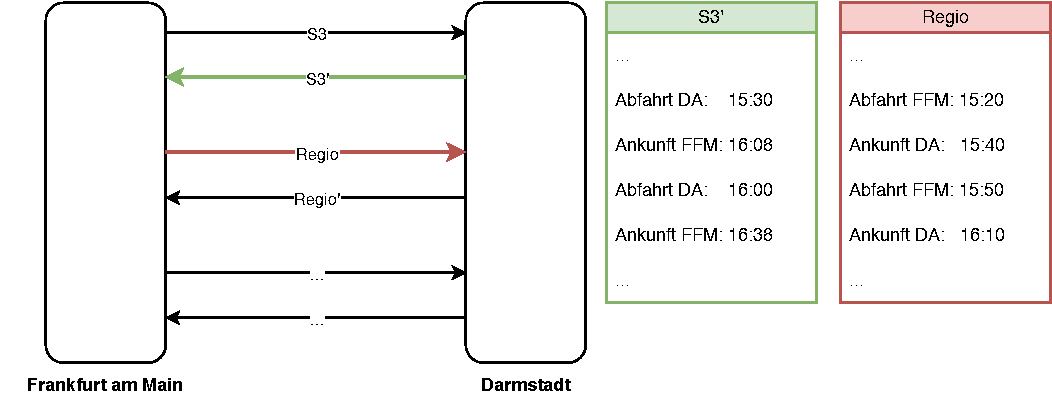
\includegraphics[width=\linewidth]{images/time-dependent/basic.pdf}
	\end{center}
\end{frame}

\begin{frame}{Das Time-Dependent Modell}
	\begin{itemize}
		\item Oder etwas formeller:
	\end{itemize}

	\begin{center}
		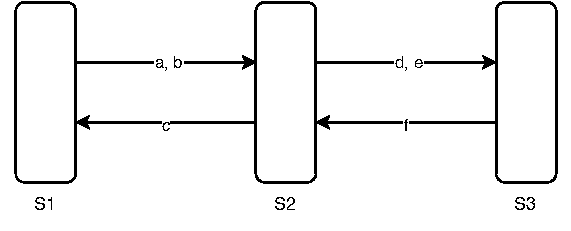
\includegraphics[width=\linewidth]{images/time-dependent/formal.pdf}
	\end{center}
\end{frame}


\begin{frame}{Das Time-Dependent Modell}
	\begin{itemize}
		\item Wir definieren für jede Kante $(u,v)$ eine\* Funktion $f(t): \mathcal{T} \rightarrow \mathcal{T}$.
		\begin{itemize}
			\item $t \in \mathcal{T}$, $\mathcal{T} \triangleq$ Zeit.
		\end{itemize}
	\end{itemize}
	\vspace{2em}
	\pause
	\begin{itemize}
		\item Dann ist unser Kantengewicht (\textit{Reisezeit}):
	\end{itemize}
	
	\begin{equation*}
		travel\_time(t) = f_{(u,v)}(t) - t
	\end{equation*}

	\vspace{4em}
	% z.B. Binärsuche auf geordneter Liste assoziiert mit {a, b} an Abfahrtszeiten von a
	\begin{block}{Frage}
		Wie sieht so eine Funktion in der Realität aus?
	\end{block}
\end{frame}

\subsection{Umstiegszeiten}
\begin{frame}{Das Time-Dependent Modell}
	\framesubtitle{Konstante Umstiegszeiten}
	\begin{itemize}
		\item Für konstante Umstiegszeiten definieren wir Zugrouten:
		\begin{itemize}
			\item Sei R eine Zugroute $S_0,S_1,...,S_{k - 1}, S_k$ für $k > 0$
			\pause
			\item Erlaubt: $S_i = S_j$, $i,j \in k$, für $i \neq j$ (Schleifen)!
		\end{itemize}
	\end{itemize}
	
	\begin{center}
		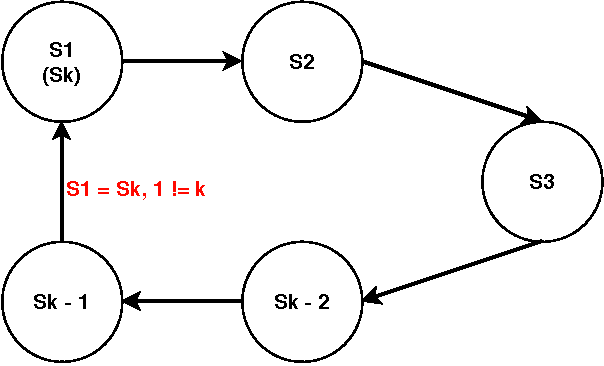
\includegraphics[height=12em]{images/time-dependent/zugroute.pdf}
	\end{center}
\end{frame}


\begin{frame}{Das Time-Dependent Modell}
	\framesubtitle{Konstante Umstiegszeiten}
	\begin{itemize}
		\item Jetze gruppieren wir alle Züge, die die gleiche Strecke fahren, in eine Zugroute
		\item \textbf{Was ist hier das Problem?}
	\end{itemize}
	
	\begin{center}
		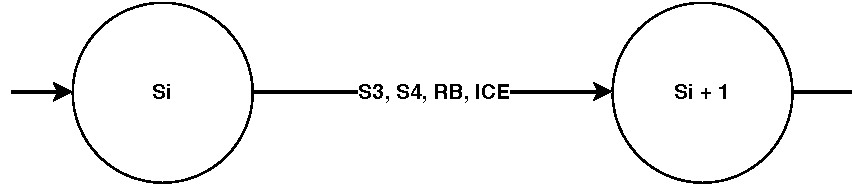
\includegraphics[width=\linewidth]{images/time-dependent/zugroute-problem.pdf}
	\end{center}
\end{frame}


\begin{frame}{Das Time-Dependent Modell}
	\framesubtitle{Konstante Umstiegszeiten}

	\begin{center}
		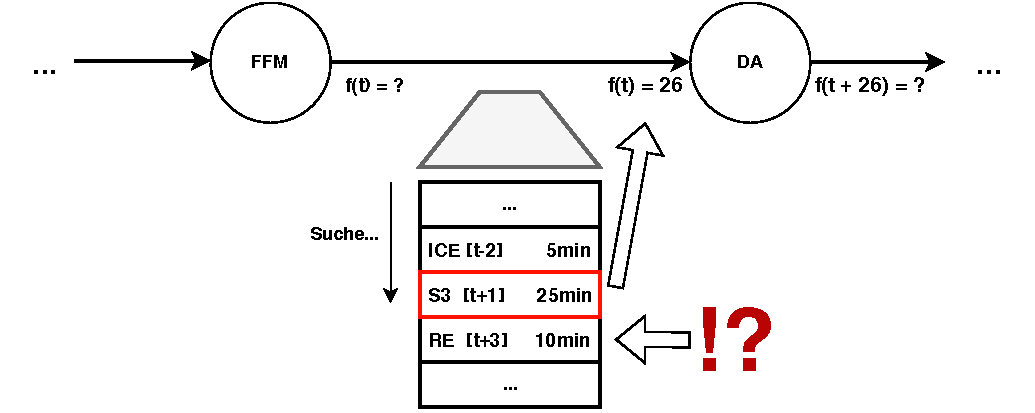
\includegraphics[width=.98\linewidth]{images/time-dependent/zugroute-problem-beispiel.pdf}
	\end{center}
	\vspace{2em}
	\pause
	\begin{block}{}
		In welchen Fällen aber wäre es doch besser, die S3 zu nehmen?
	\end{block}
\end{frame}


\begin{frame}{Das Time-Dependent Modell}
	\framesubtitle{Konstante Umstiegszeiten}
	\begin{itemize}
		\item Keine Züge $z_1,z_2$ dürfen $S_i$ um $t_1,t_2$ ($t_1 \leq t_2$) verlassen, und $z_2$ vor $z_1$ $S_{i + 1}$ erreichen!
		\item In diesem Fall spalten wir in einzelne Routen:
	\end{itemize}
	
	\begin{center}
		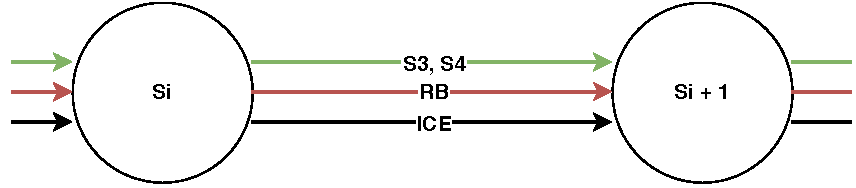
\includegraphics[width=\linewidth]{images/time-dependent/zugroute-loesung.pdf}
	\end{center}
\end{frame}


\begin{frame}{Das Time-Dependent Modell}
	\framesubtitle{Konstante Umstiegszeiten}
	\begin{itemize}
		\item Wir teilen eine Station in einen Stationsknoten $S$ und Routenknoten $r_i$
	\end{itemize}
	
	\begin{center}
		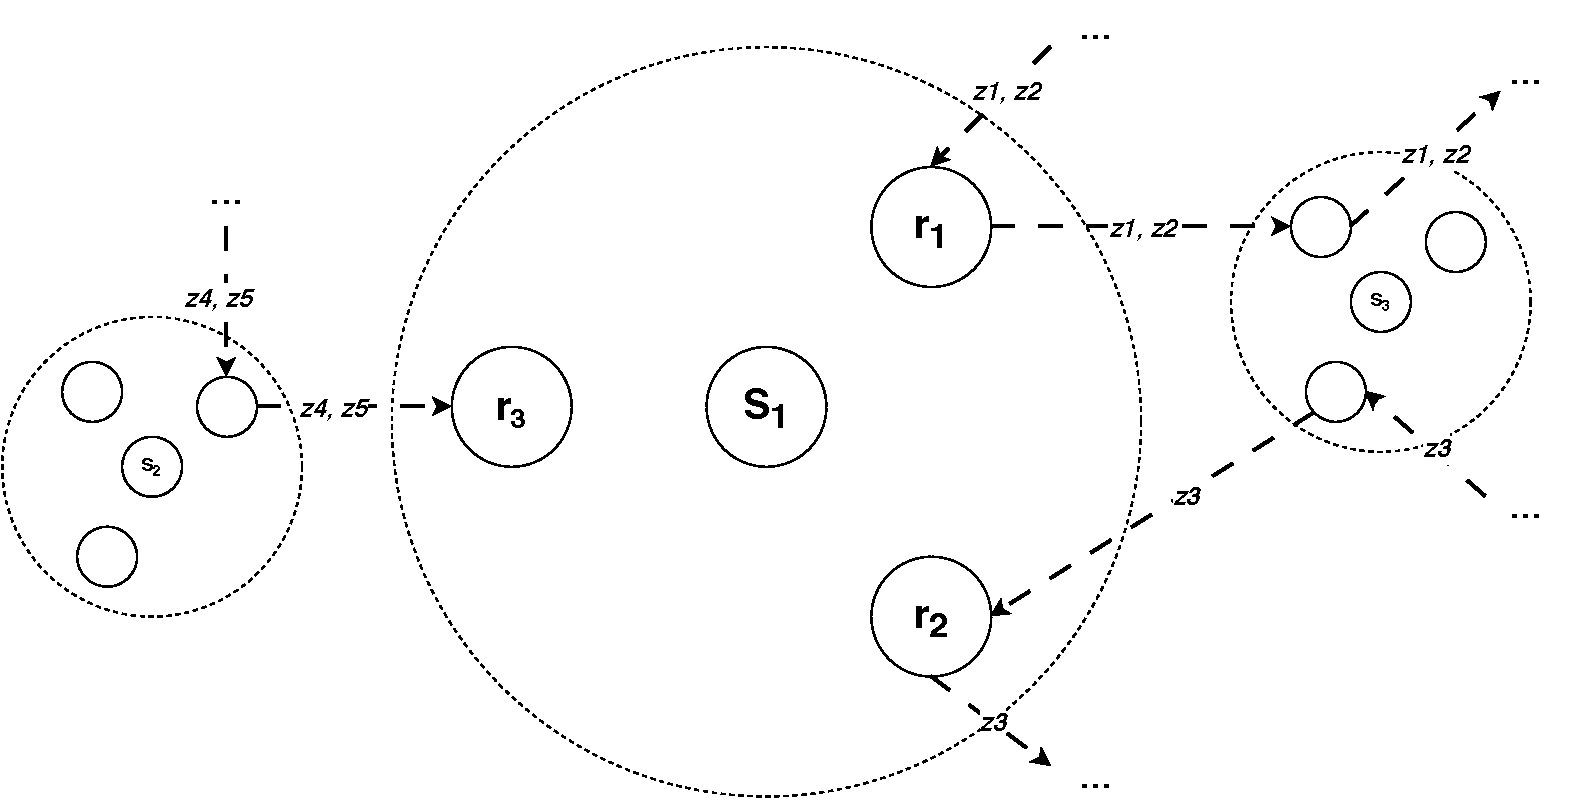
\includegraphics[width=.90\linewidth]{images/time-dependent/model_0.pdf}
	\end{center}
\end{frame}


\begin{frame}{Das Time-Dependent Modell}
	\framesubtitle{Konstante Umstiegszeiten}
	\begin{itemize}
		\item Wir erstellen Transferkanten mit \textit{ausgehenden} Transferkosten
	\end{itemize}

	% Ausgehende Kosten, optimierung, da die r-knoten den gleichen labelwert haben wie s
	% Daher können wir sie erstmal ignorieren (minimale prio) bzw erstmal komplett weglassen
	% dann später wieder einfügen
	\begin{center}
		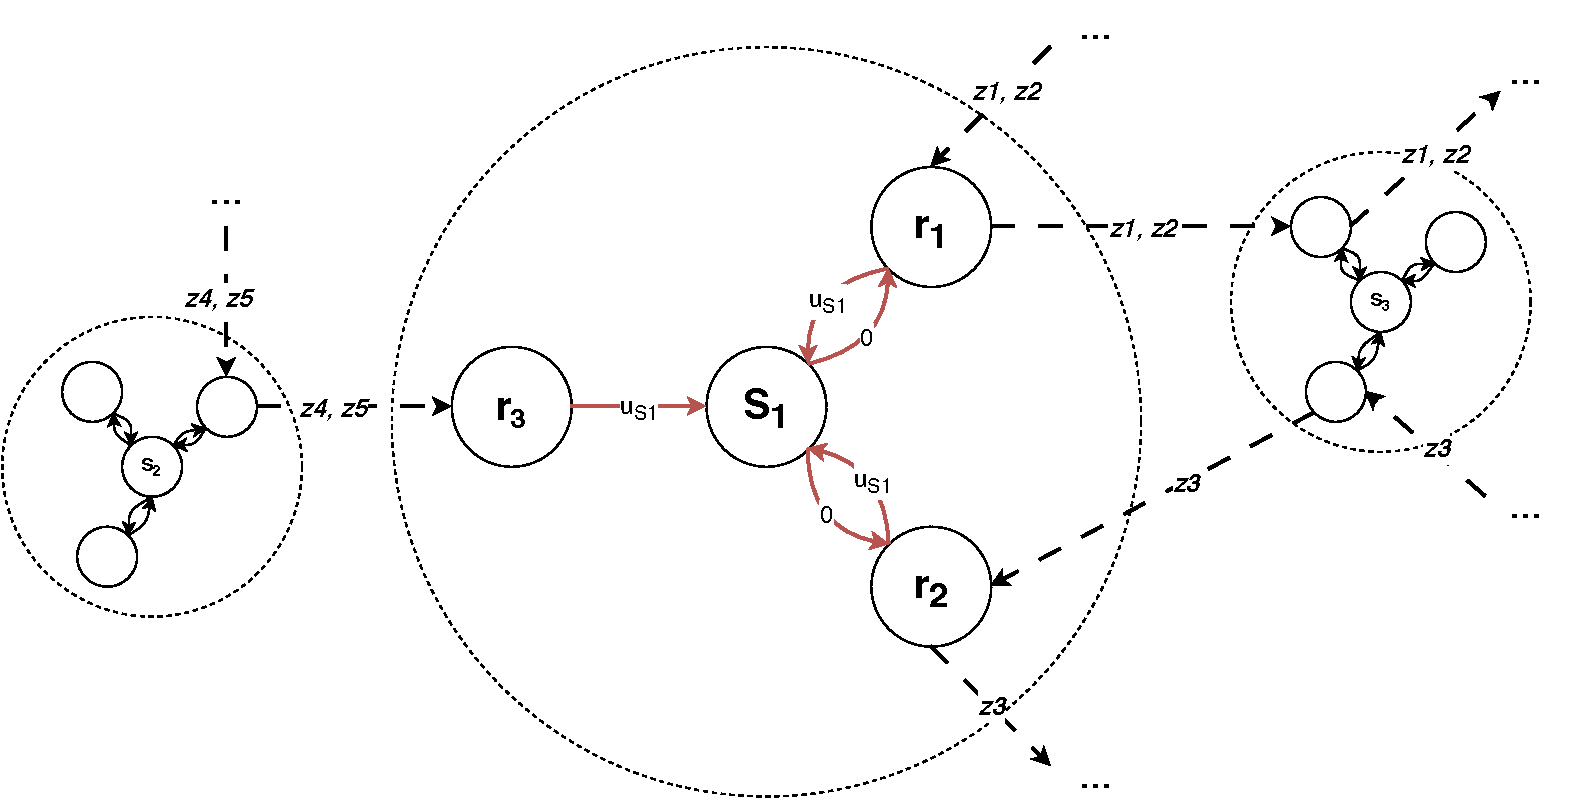
\includegraphics[width=.90\linewidth]{images/time-dependent/model_1.pdf}
	\end{center}
\end{frame}


\begin{frame}{Das Time-Dependent Modell}
	\framesubtitle{Variable Umstiegszeiten}
	\begin{itemize}
		\item Wir erstellen spezielle Kanten und Regeln zwischen Knoten
	\end{itemize}

	\begin{center}
		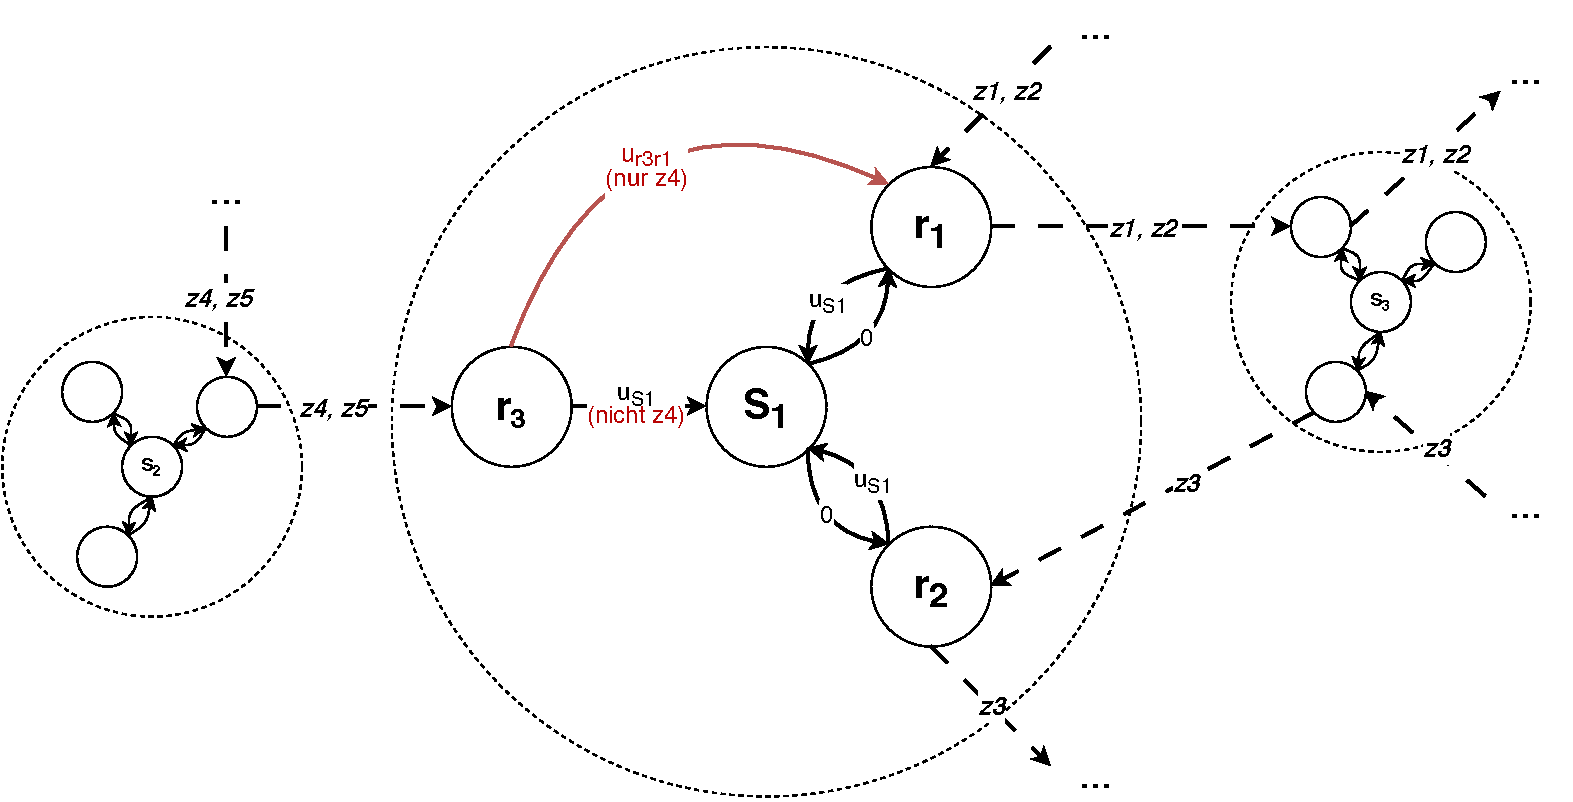
\includegraphics[width=.90\linewidth]{images/time-dependent/model_2.pdf}
	\end{center}
\end{frame}

\subsection{Verfeinerungen}
\begin{frame}{Fußwege}
	\begin{itemize}
		\item Fußwege sind immer abhängig von der Zeit, also einfach zu modellieren
	\end{itemize}

	\begin{center}
		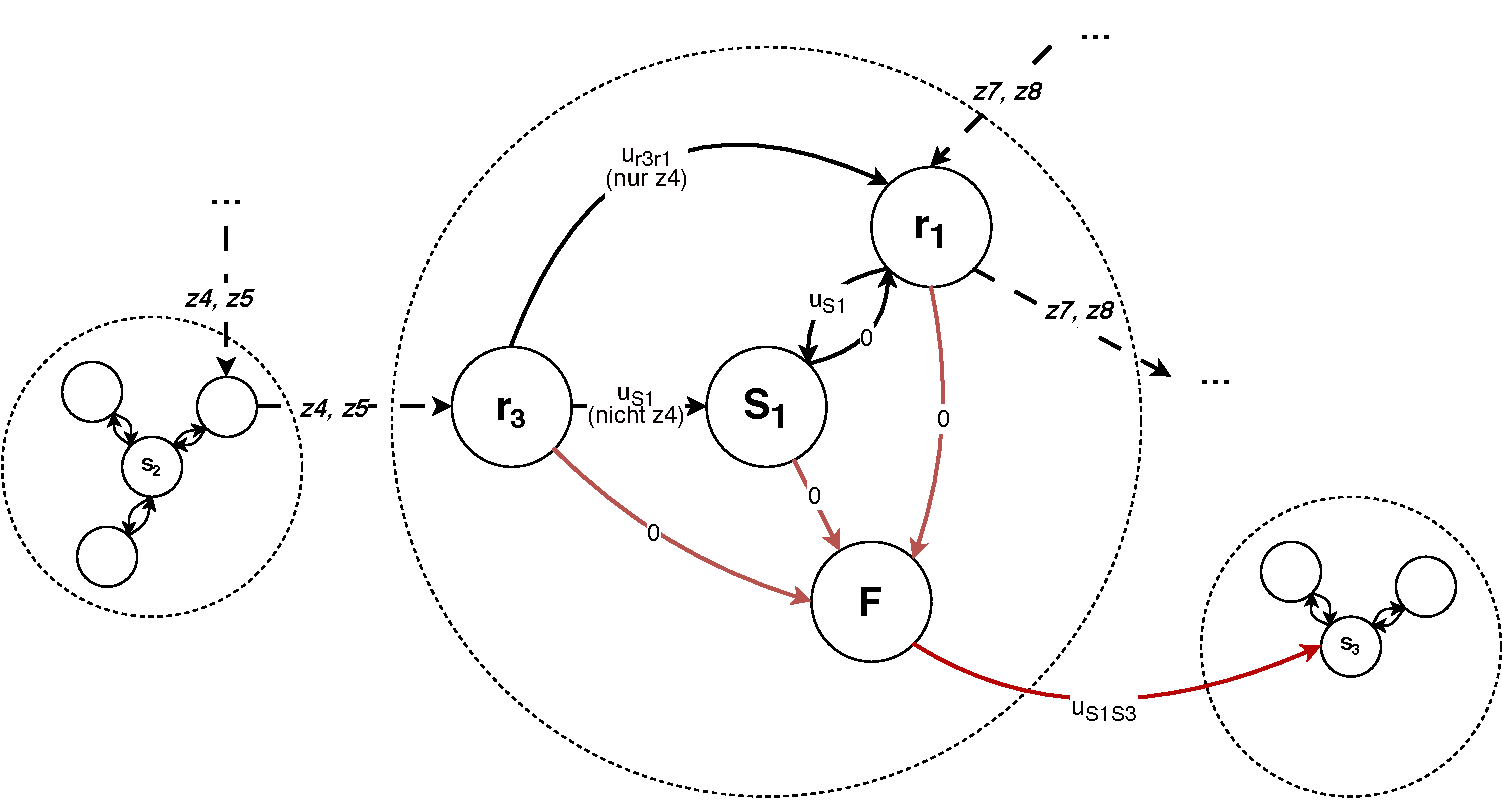
\includegraphics[width=.90\linewidth]{images/time-dependent/model_3.pdf}
	\end{center}
\end{frame}

















